% *********************************************************************
% © 2010–2026 Jeremy Sylvestre
%
% Permission is granted to copy, distribute and/or modify this document
% under the terms of the GNU Free Documentation License, Version 1.3 or
% any later version published by the Free Software Foundation; with no
% Invariant Sections, no Front-Cover Texts, and no Back-Cover Texts. A
% copy of the license is included in the appendix entitled “GNU Free
% Documentation License” that appears in the output document of this
% PreTeXt source code. All trademarks™ are the registered® marks of
% their respective owners.
%
% *********************************************************************

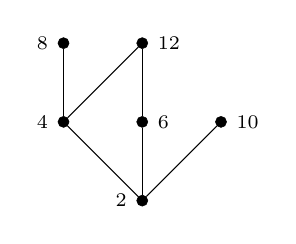
\begin{tikzpicture}[
	vertex/.style={ circle, draw, very thin, fill, inner sep=0pt, minimum size=4pt },
	vertexg/.style={ black!40!white, circle, draw, very thin, fill, inner sep=0pt, minimum size=4pt },
	vertexo/.style={ circle, draw, very thin, inner sep=0pt, minimum size=4pt }
]

\node at (1,1) (ten) [vertex,label=right:$\scriptstyle 10$] {};
\node at (-1,2) (eight) [vertex,label=left:$\scriptstyle 8$] {};
\node at (0,2) (twelve) [vertex,label=right:$\scriptstyle 12$] {};
\node at (-1,1) (four) [vertex,label=left:$\scriptstyle 4$] {};
\foreach \p in {eight,twelve} \draw (four) to (\p);
\node at (0,1) (six) [vertex,label=right:$\scriptstyle 6$] {};
\foreach \p in {twelve} \draw (six) to (\p);
\node at (0,0) (two) [vertex,label=left:$\scriptstyle 2$] {};
\foreach \p in {four,six,ten} \draw (two) to (\p);

\end{tikzpicture}
